\chapter{Cuerdas cerradas, emparejamiento de niveles y dualidad}

\lectureoverview{Una cuerda cerrada admite ondas independientes en sus dos direcciones intrínsecas. Al cuantizarlas, en un primer momento parece que se duplica el fotón de la cuerda abierta, pero la invariancia ante el desplazamiento del origen de la coordenada de la cuerda elimina los estados que solo ocupan uno de los sectores. El primer nivel que sobrevive contiene una partícula sin masa de espín dos. La misma idea de cambiar de descripción abre entonces una pregunta más amplia: cuando varían los acoplamientos, ¿qué significa que un objeto sea fundamental?}

\section{Un generador reservado}

Antes de dibujar una cuerda cerrada, recuperemos un hecho de la mecánica canónica. Supongamos que
\begin{equation}
  L=L(q_i,\dot q_i),
\end{equation}
y definamos el momento conjugado a \(q_i\) mediante
\begin{equation}
  p_i=\frac{\partial L}{\partial\dot q_i}.
\end{equation}
Una transformación continua infinitesimal puede escribirse como
\begin{equation}
  \delta q_i=\epsilon f_i(q),
  \label{eq:l04-infinitesimal-transformation}
\end{equation}
donde \(\epsilon\) es un parámetro pequeño. Si esta transformación es una simetría, el teorema de Noether proporciona una carga conservada. Al dividir el desplazamiento de la coordenada por el parámetro común se obtiene el generador
\begin{equation}
  Q=\sum_i p_i f_i(q)
   =\frac{1}{\epsilon}\sum_i p_i\,\delta q_i.
  \label{eq:l04-noether-charge}
\end{equation}
En mecánica cuántica, \(Q\) es el operador que genera la transformación pequeña correspondiente.

Una rotación en el plano \(xy\) es el ejemplo habitual. Con una elección de orientación,
\begin{equation}
  \delta x=\epsilon y,
  \qquad
  \delta y=-\epsilon x,
\end{equation}
y \eqref{eq:l04-noether-charge} se convierte en el momento angular, salvo por la misma elección de signo. El ejemplo concreto no será importante. Lo que importa es el patrón: el momento contraído con el desplazamiento infinitesimal da el generador.

\begin{figure}[H]
  \centering
  \includegraphics[width=0.76\textwidth]{lecture_04_figure_01.png}
  \caption{El momento canónico y el generador de Noether que retomaremos más adelante para el desplazamiento de la coordenada de la cuerda cerrada.}
  \lectureframe{00:05:00}
  \label{fig:l04-noether-board}
\end{figure}

Pronto encontraremos una simetría cuya coordenada no es un punto del espacio ordinario, sino la etiqueta de los puntos a lo largo de una cuerda. La ecuación
\eqref{eq:l04-noether-charge} queda aquí a mano para ese propósito.

\section{Una coordenada alrededor de un lazo}

Una cuerda cerrada no tiene extremos. Elijamos un parámetro
\begin{equation}
  0\leq \sigma<2\pi
\end{equation}
y, por el momento, marquemos un punto como \(\sigma=0\). El punto diametralmente opuesto es \(\sigma=\pi\); un cuarto de vuelta y tres cuartos de vuelta corresponden a \(\pi/2\) y \(3\pi/2\). La marca establece una convención de coordenadas, pero todavía no una característica física.

\begin{figure}[H]
  \centering
  \begin{minipage}[t]{0.58\textwidth}
    \centering
    \includegraphics[width=\textwidth]{lecture_04_figure_02.png}
    \par\smallskip\footnotesize (a) El lazo marcado en la pizarra.
  \end{minipage}\hfill
  \begin{minipage}[t]{0.37\textwidth}
    \centering
    \begin{adjustbox}{max width=\linewidth}
    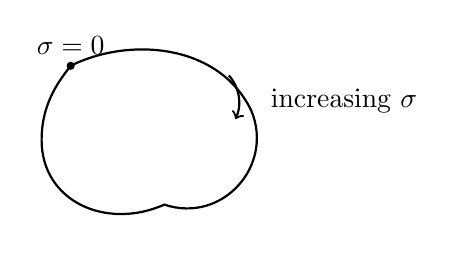
\begin{tikzpicture}[scale=0.82]
      \draw[thick]
        (0.1,1.1)
        .. controls (1.0,1.55) and (2.4,1.45) .. (2.9,0.4)
        .. controls (3.25,-0.45) and (2.45,-1.35) .. (1.55,-1.05)
        .. controls (0.65,-1.45) and (-0.35,-1.0) .. (-0.35,-0.05)
        .. controls (-0.35,0.55) and (-0.05,0.9) .. (0.1,1.1);
      \fill (0.1,1.1) circle (1.8pt);
      \node[above] at (0.1,1.12) {\(\sigma=0\)};
      \draw[->,thick] (2.55,0.95) arc[start angle=42,end angle=-25,radius=0.62];
      \node[right] at (3.05,0.55) {increasing \(\sigma\)};
    \end{tikzpicture}
    \end{adjustbox}
    \par\smallskip\footnotesize (b) La orientación intrínseca.
  \end{minipage}
  \caption{Se marca un punto para definir el origen y una flecha fija el sentido en que aumenta \(\sigma\).}
  \lectureframe{00:06:48}
  \label{fig:l04-closed-string-origin}
\end{figure}

La flecha a lo largo del lazo indica una orientación \emph{intrínseca}. No debe confundirse con el movimiento en sentido horario o antihorario en el plano \(xy\). Imaginemos que levantamos de la pizarra una banda elástica marcada, le damos la vuelta y la volvemos a colocar. El sentido horario aparente se invierte, pero la secuencia de sus marcas intrínsecas no. Lo que aumenta en \(\sigma\) sigue aumentando en \(\sigma\).

Esta distinción determina cómo hablamos de ondas que se propagan hacia la derecha y hacia la izquierda. En este capítulo, una perturbación que se propaga hacia la derecha es la que avanza hacia valores crecientes de \(\sigma\), y una que se propaga hacia la izquierda avanza hacia valores decrecientes de \(\sigma\). Ninguno de estos nombres indica en qué sentido parece moverse la perturbación en la sala.

La orientación tenía un papel concreto en el modelo original de cuerdas hadrónicas. Al romperse un tubo de flujo orientado, se produce un quark en un extremo y un antiquark en el otro; la flecha intrínseca distingue ambos extremos. También pueden construirse teorías de cuerdas no orientadas, pero en esta exposición conservaremos la flecha y los dos sentidos a lo largo de ella.

\section{Periodicidad y ondas viajeras}

Sean \(X(\sigma,\tau)\) y \(Y(\sigma,\tau)\) dos coordenadas transversales de la cuerda, y denotemos el tiempo por \(\tau\). Las coordenadas transversales adicionales, si las hay, se tratan exactamente del mismo modo. Puesto que \(\sigma=0\) y \(\sigma=2\pi\) etiquetan el mismo punto,
\begin{equation}
  X(\sigma+2\pi,\tau)=X(\sigma,\tau),
  \qquad
  Y(\sigma+2\pi,\tau)=Y(\sigma,\tau).
  \label{eq:l04-periodicity}
\end{equation}

\begin{figure}[H]
  \centering
  \includegraphics[width=0.76\textwidth]{lecture_04_figure_03.png}
  \caption{Condiciones de contorno periódicas para las dos coordenadas transversales.}
  \lectureframe{00:12:40}
  \label{fig:l04-periodicity-board}
\end{figure}

Por tanto, una ondulación localizada puede circular indefinidamente. Cuando llega a \(2\pi\), reaparece sin más en \(0\). Esto difiere de lo que ocurre en una cuerda abierta, donde una onda viajera llega a un extremo y se refleja: lo que se propagaba hacia la izquierda pasa a propagarse hacia la derecha, y viceversa. Las ondas estacionarias son naturales en una cuerda abierta, mientras que una cuerda cerrada admite dos familias que se propagan de manera independiente.

\subsection{Modos de Fourier complejos}

La base conveniente para una función periódica es
\begin{equation}
  e^{in\sigma}=\cos(n\sigma)+i\sin(n\sigma),
  \qquad n\in\mathbb Z.
\end{equation}
La condición de que el índice sea entero viene impuesta por la periodicidad:
\(e^{in(\sigma+2\pi)}=e^{in\sigma}\). Por ejemplo, sustituir \(n\) por un semientero haría que la función cambiara tras una vuelta completa.

Si por el momento omitimos la dependencia temporal, la expansión en la pizarra es
\begin{align}
  X(\sigma)
  &=
  X_0+
  \sum_{n>0}X_n e^{in\sigma}
  +\sum_{n>0}X_{-n}e^{-in\sigma},
  \label{eq:l04-fourier-x}\\
  Y(\sigma)
  &=
  Y_0+
  \sum_{n>0}Y_n e^{in\sigma}
  +\sum_{n>0}Y_{-n}e^{-in\sigma}.
  \label{eq:l04-fourier-y}
\end{align}
Para \(X\) y \(Y\) reales, en el nivel clásico los coeficientes de índice negativo son los conjugados complejos de los coeficientes de índice positivo. Los modos cero \(X_0\) y \(Y_0\) localizan el centro de masas; son posiciones, no oscilaciones internas.

\begin{figure}[H]
  \centering
  \includegraphics[width=0.82\textwidth]{lecture_04_figure_04.png}
  \caption{Las partes de índices positivo y negativo de la expansión de Fourier periódica, seguidas del modo cero.}
  \lectureframe{00:20:00}
  \label{fig:l04-fourier-board}
\end{figure}

\begin{classroomqa}
\audiencequestion{Si son ondas viajeras, ¿dónde está la coordenada temporal?\lecturetimestamp{00:19:05}}
\lecturerresponse{Solo se ha omitido en la notación de la pizarra. Una solución viajera lleva una fase que depende tanto de \(\sigma\) como de \(\tau\). Con la convención que usaremos más adelante, una familia tiene
\(e^{-in(\tau-\sigma)}\) y la otra
\(e^{-in(\tau+\sigma)}\).}
\end{classroomqa}

Así pues, lo que determina la propagación es la fase completa, no el signo de \(n\) en un factor de Fourier puramente espacial por sí solo. Podemos escribir
\begin{equation}
  X(\sigma,\tau)=X_R(\tau-\sigma)+X_L(\tau+\sigma),
  \label{eq:l04-chiral-solution}
\end{equation}
y, de manera análoga, para \(Y\). Llamar \(R\) a una familia en vez de \(L\) es una convención; el hecho invariante es que hay dos sentidos opuestos a lo largo del círculo de \(\sigma\).\editorialnote{Un factor \(e^{in\sigma}\) en un instante dado no especifica por sí solo una onda viajera. La propagación queda determinada solo cuando se da la fase temporal.}

\section{Energía en los dos sentidos}

La dinámica local es la misma que en la cuerda abierta. Con la normalización simplificada que usamos aquí,
\begin{equation}
  L\propto
  \int_0^{2\pi}d\sigma\,
  \left[
    \dot X^2-X'^2+\dot Y^2-Y'^2
  \right],
  \label{eq:l04-string-lagrangian}
\end{equation}
donde un punto denota \(\partial_\tau\) y una prima denota \(\partial_\sigma\). La energía tiene un signo más entre los términos cinético y elástico:
\begin{equation}
  E\propto
  \int_0^{2\pi}d\sigma\,
  \left[
    \dot X^2+X'^2+\dot Y^2+Y'^2
  \right].
  \label{eq:l04-string-energy}
\end{equation}
Para cualquiera de las dos coordenadas transversales,
\begin{equation}
  \dot X^2+X'^2
  =
  \frac12(\dot X+X')^2+
  \frac12(\dot X-X')^2.
  \label{eq:l04-energy-square-completion}
\end{equation}
Los términos cruzados se cancelan y quedan exactamente las energías cinética y de gradiente originales.

\begin{figure}[H]
  \centering
  \includegraphics[width=0.82\textwidth]{lecture_04_figure_05.png}
  \caption{La energía total reorganizada en los dos sectores de ondas viajeras.}
  \lectureframe{00:25:10}
  \label{fig:l04-energy-board}
\end{figure}

Para \(X_R(\tau-\sigma)\), se cumple \(\dot X_R=-X_R'\); para \(X_L(\tau+\sigma)\), se cumple \(\dot X_L=X_L'\). Por consiguiente, los dos cuadrados de \eqref{eq:l04-energy-square-completion} aíslan las dos familias quirales. Incluyendo todas las coordenadas transversales, definamos
\begin{align}
  E_L&\propto
  \frac12\int_0^{2\pi}d\sigma
  \sum_I(\dot X^I+X^{I\prime})^2,\\
  E_R&\propto
  \frac12\int_0^{2\pi}d\sigma
  \sum_I(\dot X^I-X^{I\prime})^2.
  \label{eq:l04-left-right-energies}
\end{align}
Entonces \(E=E_L+E_R\). Como las ecuaciones son lineales en esta etapa, las ondas de los dos sectores se atraviesan sin dispersarse.

\subsection{El doble de osciladores}

Al sustituir la serie de Fourier en \eqref{eq:l04-string-lagrangian}, cada coeficiente de modo no nulo se convierte en un oscilador armónico. Su frecuencia es proporcional a \(|n|\): una longitud de onda menor implica una frecuencia mayor y, por tanto, una energía de excitación más alta. A diferencia de lo que ocurre en la cuerda abierta, cada frecuencia positiva aparece en dos copias que se propagan de manera independiente.

En la pizarra, los operadores de creación polarizados en \(X\) son \(a_n^+\) y \(a_{-n}^+\), y los polarizados en \(Y\) son \(b_n^+\) y \(b_{-n}^+\). Para separar con mayor claridad la creación de la propagación, escribiremos
\begin{equation}
  a_n^\dagger,\quad b_n^\dagger,
  \qquad
  \widetilde a_n^\dagger,\quad\widetilde b_n^\dagger,
  \qquad n>0.
  \label{eq:l04-oscillator-notation}
\end{equation}
Los operadores sin tilde y con tilde crean modos que se propagan en sentidos opuestos sobre la hoja de universo; \(a\) y \(b\) denotan las dos polarizaciones transversales.

\begin{figure}[H]
  \centering
  \includegraphics[width=0.65\textwidth]{lecture_04_figure_06.png}
  \caption{La notación de la pizarra para los operadores de creación duplicados, polarizados en \(X\) y \(Y\).}
  \lectureframe{00:29:10}
  \label{fig:l04-oscillators-board}
\end{figure}

Si \(N_n^{(a)},N_n^{(b)}\) y sus correspondientes operadores con tilde son números de ocupación, los niveles de oscilación en los dos sentidos son, esquemáticamente,
\begin{equation}
  \begin{aligned}
    N&=\sum_{n>0}n\bigl(N_n^{(a)}+N_n^{(b)}+\cdots\bigr),\\
    \widetilde N&=\sum_{n>0}n
      \bigl(\widetilde N_n^{(a)}+\widetilde N_n^{(b)}+\cdots\bigr).
  \end{aligned}
  \label{eq:l04-level-operators}
\end{equation}
Los puntos suspensivos representan las direcciones transversales adicionales.

\section{La conjetura sobre el espectro que falla}

Recordemos el primer nivel de la cuerda abierta. Al actuar sobre el estado fundamental con \(a_1^\dagger\) o \(b_1^\dagger\) se obtienen dos polarizaciones lineales. Sus combinaciones circulares,
\begin{equation}
  c_\pm^\dagger
  =
  \frac{1}{\sqrt2}
  \left(a_1^\dagger\pm i b_1^\dagger\right),
  \label{eq:l04-open-circular}
\end{equation}
tienen helicidad \(h=\pm1\). La ausencia de un estado asociado de helicidad cero es la señal de un vector sin masa en esta descripción elemental en cuatro dimensiones.

Sea \(m_0^2\) la masa al cuadrado del estado fundamental de la cuerda cerrada. Una primera conjetura ingenua consiste en actuar una vez con cualquiera de los operadores de
\begin{equation}
  a_1^\dagger,\quad b_1^\dagger,\quad
  \widetilde a_1^\dagger,\quad\widetilde b_1^\dagger.
  \label{eq:l04-naive-one-sided}
\end{equation}
Esto se parece a dos copias del fotón de la cuerda abierta, una por cada sentido de propagación. Sin embargo, a la energía siguiente, la lista sin restricciones no se organiza en multipletes de rotación coherentes. El problema no se resuelve con un tratamiento más elaborado. La premisa de que todo monomio de osciladores es un estado físico es incorrecta.

\subsection{Emparejamiento de niveles: primero, como regla}

La condición física de la cuerda cerrada es
\begin{equation}
  N=\widetilde N,
  \qquad\text{equivalently}\qquad E_L=E_R.
  \label{eq:l04-level-matching}
\end{equation}
Por ahora, tomémosla como un postulado; deduciremos su origen solo después de ver qué consigue.

Todos los estados de \eqref{eq:l04-naive-one-sided} tienen una unidad de energía en un sector y ninguna en el otro, de modo que quedan excluidos. Los primeros estados que sobreviven contienen un oscilador de cada familia:
\begin{align}
  a_1^\dagger\widetilde a_1^\dagger\ket{0},
  &\qquad
  b_1^\dagger\widetilde b_1^\dagger\ket{0},
  \label{eq:l04-four-matched-a}\\
  a_1^\dagger\widetilde b_1^\dagger\ket{0},
  &\qquad
  b_1^\dagger\widetilde a_1^\dagger\ket{0}.
  \label{eq:l04-four-matched-b}
\end{align}
Su energía total de oscilación es dos, repartida por igual entre los dos sentidos. Un único operador de creación \(n=2\) tiene la misma energía total de oscilación, pero no satisface \eqref{eq:l04-level-matching}: aporta dos unidades a un solo lado.

\begin{figure}[H]
  \centering
  \includegraphics[width=0.70\textwidth]{lecture_04_figure_07.png}
  \caption{Los cuatro estados del primer nivel que sobreviven al emparejamiento de niveles. En la pizarra se usan los subíndices \(1\) y \(-1\) donde \eqref{eq:l04-four-matched-a}--\eqref{eq:l04-four-matched-b} usa operadores sin tilde y con tilde.}
  \lectureframe{00:41:05}
  \label{fig:l04-level-matched-board}
\end{figure}

\section{Un gravitón en el primer nivel emparejado}

Expresemos las dos familias quirales en una base circular:
\begin{equation}
  c_\pm^\dagger
  =\frac{a_1^\dagger\pm i b_1^\dagger}{\sqrt2},
  \qquad
  \widetilde c_\pm^\dagger
  =\frac{\widetilde a_1^\dagger\pm i\widetilde b_1^\dagger}{\sqrt2}.
  \label{eq:l04-closed-circular}
\end{equation}
Cada factor aporta una helicidad \(+1\) o \(-1\) en el espacio transversal ordinario. Por tanto, sus productos dan
\begin{center}
\begin{tabular}{c c}
  \toprule
  Estado & Hel icidad \\
  \midrule
  \(c_+^\dagger\widetilde c_+^\dagger\ket0\) & \(+2\) \\
  \(c_-^\dagger\widetilde c_-^\dagger\ket0\) & \(-2\) \\
  \(c_+^\dagger\widetilde c_-^\dagger\ket0\) & \(0\) \\
  \(c_-^\dagger\widetilde c_+^\dagger\ket0\) & \(0\) \\
  \bottomrule
\end{tabular}
\end{center}

\begin{classroomqa}
\audiencequestion{¿El segundo factor de polarización circular debe provenir del sector de propagación opuesto?\lecturetimestamp{00:43:20}}
\lecturerresponse{Sí. La primera expresión escrita en la pizarra se corrigió precisamente por este motivo. Aquí, un estado físico debe emparejar un oscilador que se propaga hacia la derecha con otro que se propaga hacia la izquierda; de lo contrario, no satisface el emparejamiento de niveles. Las helicidades se refieren a la polarización en el espacio transversal, mientras que los dos factores corresponden a sentidos opuestos sobre la hoja de universo.}
\end{classroomqa}

\begin{figure}[H]
  \centering
  \includegraphics[width=0.82\textwidth]{lecture_04_figure_08.png}
  \caption{Los cuatro productos en la base circular tras la corrección de la pizarra, con helicidades \(+2,-2,0,0\).}
  \lectureframe{00:46:10}
  \label{fig:l04-helicity-board}
\end{figure}

Una partícula masiva de espín dos tiene cinco proyecciones del espín,
\begin{equation}
  m=2,1,0,-1,-2.
\end{equation}
El nivel emparejado no contiene estados asociados con \(m=\pm1\). Por tanto, no puede formar un multiplete de espín dos masivo. En cambio, una partícula sin masa de espín dos tiene solo las helicidades \(+2\) y \(-2\). Los productos de igual helicidad son precisamente esos dos estados: las polarizaciones del gravitón.

Quedan dos combinaciones de helicidad cero. En el lenguaje usado en clase, una es el dilatón y la otra el axión. Una descripción covariante de la cuerda bosónica cerrada genérica precisa esta afirmación:
\begin{equation}
  \begin{aligned}
    \alpha_{-1}^{I}\widetilde\alpha_{-1}^{J}\ket{0;k}
    &\longrightarrow
    \underbrace{h_{IJ}}_{\text{symmetric traceless}}
    \oplus
    \underbrace{B_{IJ}}_{\text{antisymmetric}}\\
    &\hspace{2.5em}\oplus
    \underbrace{\Phi}_{\text{trace}}.
  \end{aligned}
  \label{eq:l04-massless-tensor-decomposition}
\end{equation}
Estos son el gravitón, la forma diferencial antisimétrica de dos índices y el dilatón. En cuatro dimensiones, la forma de dos índices puede dualizarse a un pseudoescalar similar a un axión, que es el lenguaje adoptado en la clase.\editorialnote{El segundo estado de helicidad cero es, fundamentalmente, el campo tensorial antisimétrico \(B_{\mu\nu}\) del espectro genérico de cuerdas cerradas. Llamarlo axión corresponde a la descripción dual en cuatro dimensiones.}

En este nivel formal, los tres campos no tienen masa. La compactificación, las proyecciones y la dinámica del fondo pueden alterar cuáles grados de libertad escalares o de dos índices siguen siendo ligeros. El gravitón es distinto: una vez que existe un sector de cuerdas cerradas con interacciones coherentes, su estado sin masa de espín dos es inevitable. Por eso la gravedad emerge de las cuerdas cerradas en vez de añadirse como ingrediente separado.

\section{Por qué deben coincidir los niveles}

Volvamos ahora a la marca en \(\sigma=0\). ¿Es una cuenta física unida al lazo o solo el origen de nuestro parámetro? En una cuerda cerrada ordinaria sin marcar, ningún punto debe ser privilegiado. El estado cuántico debe permanecer inalterado cuando se desplazan a la vez todas las etiquetas.

\subsection{La versión discreta}

Regularicemos el lazo como \(M\) puntos ordenados con coordenadas transversales \((X_i,Y_i)\). Omitamos temporalmente \(Y_i\). Una función de onda en el espacio de configuraciones es
\begin{equation}
  \Psi(X_1,X_2,\ldots,X_M).
\end{equation}
Cambiar qué punto se considera primero da una permutación cíclica:
\begin{align}
  \Psi(X_1,X_2,\ldots,X_M)
  &=
  \Psi(X_2,\ldots,X_M,X_1)\nonumber\\
  &=
  \Psi(X_3,\ldots,X_M,X_1,X_2).
  \label{eq:l04-cyclic-wavefunction}
\end{align}
Esto no es invariancia ante una permutación arbitraria. Por ejemplo, insertar \(X_3\) entre \(X_1\) y \(X_2\) cambia la estructura de adyacencia y, en la práctica, corta y vuelve a conectar la cuerda discretizada. Solo el cambio cíclico común de etiquetas
\begin{equation}
  X_i\longrightarrow X_{i+1}\qquad(\text{mod }M)
  \label{eq:l04-discrete-shift}
\end{equation}
expresa la ausencia de un origen preferido.

\begin{figure}[H]
  \centering
  \includegraphics[width=0.82\textwidth]{lecture_04_figure_09.png}
  \caption{Las identidades cíclicas de la función de onda para una cuerda cerrada discretizada.}
  \lectureframe{00:56:20}
  \label{fig:l04-cyclic-board}
\end{figure}

\subsection{La versión del continuo}

En el límite del continuo \(M\to\infty\), el estado es el funcional de onda
\begin{equation*}
  \Psi[X(\sigma),Y(\sigma)].
\end{equation*}
Un cambio cíclico de etiquetas se convierte en
\begin{equation}
  \sigma\longrightarrow\sigma+\epsilon.
\end{equation}
La invariancia exige que
\begin{equation}
  \Psi[X(\sigma+\epsilon),Y(\sigma+\epsilon)]
  =
  \Psi[X(\sigma),Y(\sigma)].
  \label{eq:l04-wavefunctional-invariance}
\end{equation}

\begin{figure}[H]
  \centering
  \includegraphics[width=0.72\textwidth]{lecture_04_figure_10.png}
  \caption{El desplazamiento discreto y su forma continua como funcional de onda.}
  \lectureframe{00:58:40}
  \label{fig:l04-wavefunctional-board}
\end{figure}

A primer orden,
\begin{equation}
  \delta X(\sigma)=\epsilon X'(\sigma),
  \qquad
  \delta Y(\sigma)=\epsilon Y'(\sigma),
  \label{eq:l04-profile-shift}
\end{equation}
salvo el signo global que distingue un desplazamiento activo del perfil de un desplazamiento pasivo de la coordenada. La variación correspondiente del funcional de onda es
\begin{equation}
  \delta\Psi
  =
  \epsilon\int_0^{2\pi}d\sigma
  \left[
    \frac{\delta\Psi}{\delta X(\sigma)}X'(\sigma)
    +
    \frac{\delta\Psi}{\delta Y(\sigma)}Y'(\sigma)
  \right].
  \label{eq:l04-functional-variation}
\end{equation}

\begin{figure}[H]
  \centering
  \includegraphics[width=0.72\textwidth]{lecture_04_figure_11.png}
  \caption{La expansión a primer orden del argumento desplazado del funcional de onda.}
  \lectureframe{01:01:31}
  \label{fig:l04-functional-expansion-board}
\end{figure}

\begin{classroomqa}
\audiencequestion{¿La condición de primer orden es una ecuación independiente para cada valor de \(\sigma\)?\lecturetimestamp{01:01:30}}
\lecturerresponse{No. La transformación desplaza todos los puntos de la cuerda a la vez. Hay que sumar la variación en un punto a las variaciones en todos los demás; por eso la expresión continua contiene la integral sobre \(\sigma\).}
\end{classroomqa}

En la representación de coordenadas,
\begin{equation}
  P_X(\sigma)=-i\frac{\delta}{\delta X(\sigma)},
  \qquad
  P_Y(\sigma)=-i\frac{\delta}{\delta Y(\sigma)}
  \label{eq:l04-functional-momenta}
\end{equation}
con \(\hbar=1\). Por tanto, la ecuación \eqref{eq:l04-functional-variation} está generada por
\begin{equation}
  G_\sigma=
  \int_0^{2\pi}d\sigma\,
  \left[
    P_X(\sigma)X'(\sigma)+P_Y(\sigma)Y'(\sigma)
  \right].
  \label{eq:l04-sigma-generator}
\end{equation}
Este es exactamente el esquema de Noether \eqref{eq:l04-noether-charge}: el momento canónico multiplicado por el desplazamiento de la coordenada, sumado sobre todos los grados de libertad. Un estado de cuerda cerrada sin marcar satisface
\begin{equation}
  G_\sigma\ket{\mathrm{phys}}=0.
  \label{eq:l04-physical-generator-condition}
\end{equation}

Con la normalización de \eqref{eq:l04-string-lagrangian},
\(P_I\propto\dot X^I\), por lo que la misma condición se escribe
\begin{equation}
  \int_0^{2\pi}d\sigma
  \sum_I\dot X^I X^{I\prime}=0.
  \label{eq:l04-momentum-constraint}
\end{equation}

\begin{figure}[H]
  \centering
  \includegraphics[width=0.75\textwidth]{lecture_04_figure_12.png}
  \caption{El generador integrado, una vez identificado el momento con la derivada del funcional de onda.}
  \lectureframe{01:05:10}
  \label{fig:l04-generator-board}
\end{figure}

\subsection{El generador es la diferencia de energías}

La suma de las dos expresiones de \eqref{eq:l04-left-right-energies} es la energía total. Su diferencia es
\begin{align}
  E_L-E_R
  &\propto
  \frac12\int_0^{2\pi}d\sigma\sum_I
  \left[
    (\dot X^I+X^{I\prime})^2\right.\nonumber\\[-0.25em]
  &\hspace{7em}\left.
    -(\dot X^I-X^{I\prime})^2
  \right]\\
  &=
  2\int_0^{2\pi}d\sigma\sum_I
  \dot X^I X^{I\prime}.
  \label{eq:l04-energy-difference}
\end{align}
La integral es el generador que debe anular un estado físico. Por tanto,
\begin{equation}
  E_L-E_R=0,
  \qquad\text{or}\qquad
  N-\widetilde N=0.
\end{equation}
El emparejamiento de niveles expresa que el origen de la coordenada \(\sigma\) es inobservable.

\begin{figure}[H]
  \centering
  \includegraphics[width=0.78\textwidth]{lecture_04_figure_13.png}
  \caption{La suma y la diferencia de energías que se muestran juntas al final de la deducción del emparejamiento de niveles.}
  \lectureframe{01:06:40}
  \label{fig:l04-energy-difference-board}
\end{figure}

\begin{classroomqa}
\audiencequestion{¿Por qué las fórmulas mostradas parecen colocar el factor de un medio en lugares distintos?\lecturetimestamp{01:06:28}}
\lecturerresponse{Aquí solo se usa la estructura relativa. Al restablecer una normalización global coherente, aparece el factor de un medio en la identidad de cuadrados completos \eqref{eq:l04-energy-square-completion}. La suma da la energía total, mientras que la diferencia sigue siendo proporcional a \(\int d\sigma\,\dot X X'\). Su anulación y, por tanto, el emparejamiento de niveles, son independientes de esa convención común.}
\end{classroomqa}

La restricción elimina una gran parte del espectro ingenuo de osciladores, y elimina precisamente los estados que no formaban multipletes de partículas coherentes. No elimina el fotón de la cuerda abierta, porque una cuerda abierta no tiene dos sectores independientes que circulen y estén sujetos a esta condición propia de un lazo cerrado. En la cuerda cerrada, deja el gravitón, el dilatón, el estado de tensor antisimétrico o similar a un axión, y los niveles emparejados superiores.\editorialnote{En la cuantización covariante de cuerdas, el emparejamiento de niveles es la condición del modo cero \(L_0-\widetilde L_0=0\), uno de los elementos del sistema de restricciones de la hoja de universo. La deducción de aquí aísla su origen intuitivo: la invariancia ante traslaciones alrededor de la cuerda cerrada.}

\section{Dos sentidos distintos de izquierda y derecha}

Ahora hay dos usos distintos del lenguaje de orientación:
\begin{enumerate}
  \item \(X_R(\tau-\sigma)\) y \(X_L(\tau+\sigma)\) describen la propagación en sentidos opuestos a lo largo del círculo intrínseco \(\sigma\).
  \item \(c_+^\dagger\) y \(c_-^\dagger\) describen la polarización circular en el plano transversal físico \(xy\).
\end{enumerate}
El estado del gravitón que satisface el emparejamiento de niveles contiene un oscilador de cada sentido de propagación sobre la hoja de universo. Sin embargo, esos dos osciladores pueden tener la misma helicidad espaciotemporal, lo que produce \(h=+2\) o \(h=-2\). Confundir estos dos sentidos de izquierda y derecha hace que el espectro parezca contradictorio, aunque no lo sea.

\section{¿Qué significa fundamental?}

Una vez cuantizadas las cuerdas abiertas y cerradas en este nivel elemental, queda una pregunta natural: ¿son las cuerdas los constituyentes últimos o podrían estar hechas, a su vez, de algo más?

\begin{classroomqa}
\audiencequestion{¿Hay pruebas o razones para considerar que las cuerdas son los objetos más fundamentales, sin nada más pequeño por debajo de ellas?\lecturetimestamp{01:10:44}}
\lecturerresponse{No hay una respuesta útil que sea independiente del parámetro. Los grados de libertad que parecen elementales en un régimen pueden volverse pesados, extendidos y aparentemente compuestos en otro. Conviene entender «fundamental» como una afirmación sobre qué variables ofrecen una descripción útil para el acoplamiento considerado.}
\end{classroomqa}

Las cargas eléctricas y magnéticas ofrecen el ejemplo más claro de esta idea. Supongamos que una teoría contiene una carga eléctrica \(e\) y una carga magnética \(g\). La cuerda de Dirac inobservable unida a un monopolo exige que
\begin{equation}
  eg=2\pi n,
  \qquad n\in\mathbb Z.
  \label{eq:l04-dirac-quantization}
\end{equation}
Para las cargas mínimas, \(n=1\). Una partícula cargada que rodea la cuerda de Dirac adquiere entonces una fase \(e^{ieg}=1\), de modo que no es posible detectar la cuerda auxiliar.

\begin{figure}[H]
  \centering
  \begin{minipage}[t]{0.58\textwidth}
    \centering
    \includegraphics[width=\textwidth]{lecture_04_figure_14.png}
    \par\smallskip\footnotesize (a) Cuantización de Dirac en la pizarra.
  \end{minipage}\hfill
  \begin{minipage}[t]{0.36\textwidth}
    \centering
    \begin{adjustbox}{max width=\linewidth}
    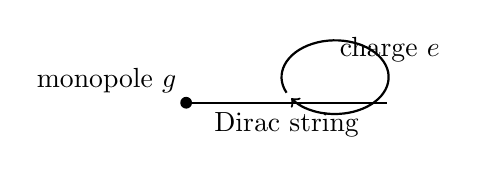
\begin{tikzpicture}[scale=0.85]
      \fill (0,0) circle (2.5pt);
      \node[above left] at (0,0) {monopole \(g\)};
      \draw[thick] (0,0) -- (3.0,0);
      \node[below] at (1.5,0) {Dirac string};
      \draw[->,thick] (1.5,0.15) arc[start angle=205,end angle=-145,
        x radius=0.8,y radius=0.55];
      \node[right] at (2.15,0.8) {charge \(e\)};
    \end{tikzpicture}
    \end{adjustbox}
    \par\smallskip\footnotesize (b) El experimento de fase alrededor de la cuerda.
  \end{minipage}
  \caption{La condición de Dirac relaciona inversamente las cargas eléctricas y magnéticas.}
  \lectureframe{01:13:20}
  \label{fig:l04-dirac-board}
\end{figure}

Si \(e\) es pequeño, resulta útil la teoría de perturbaciones ordinaria en las variables eléctricas. Los diagramas de Feynman con vértices eléctricos adicionales quedan cada vez más suprimidos. Pero \eqref{eq:l04-dirac-quantization} hace que \(g\) sea grande, por lo que no resulta útil una expansión diagramática en vértices magnéticos. En términos de los acoplamientos adimensionales habituales,
\begin{equation}
  \alpha_e=\frac{e^2}{4\pi},
  \qquad
  \alpha_m=\frac{g^2}{4\pi},
  \qquad
  \alpha_e\alpha_m=\frac{n^2}{4}.
  \label{eq:l04-dual-couplings}
\end{equation}
Un acoplamiento eléctrico débil corresponde a un acoplamiento magnético fuerte, y viceversa.

El monopolo con acoplamiento fuerte también parece complicado desde la descripción eléctrica. La energía de su campo es grande; está vestido por una nube intensa de fluctuaciones del campo gauge y de pares virtuales con carga magnética. Se comporta como un objeto pesado y extendido, un punto de partida poco apropiado para una serie perturbativa eléctrica. Esto no demuestra que sea menos fundamental. Indica que esa variable elemental es inadecuada para ese régimen.

Imaginemos ahora que aumentamos continuamente \(e\). La condición de cuantización obliga a que \(g\) disminuya. Cerca de la región autodual, ninguna de las dos descripciones es especialmente débil; más allá, las variables magnéticas pueden volverse más simples y ligeras, mientras que los objetos eléctricos quedan fuertemente vestidos. La carga que se considera elemental cambia sin que cambie el contenido físico de la teoría.

\subsection{La pregunta de Wigner}

Esta ambigüedad surgió en cierta ocasión en una discusión sobre si el bosón de Higgs era fundamental o compuesto. Eugene Wigner preguntó repetidamente qué significaba «compuesto». Una distinción propuesta se basaba en la desintegración: quizá un objeto fundamental no puede desintegrarse y uno compuesto sí. Pero un átomo de hidrógeno en su estado fundamental no puede desintegrarse y es claramente compuesto; el protón puede ser estable y el neutrón desintegrarse, pero eso no convierte a uno en elemental y al otro en compuesto en el sentido pretendido. Cada definición sencilla daba lugar a otro contraejemplo.

Gerardus 't Hooft cerró la discusión con un criterio operativo: un objeto es fundamental cuando resulta útil considerarlo fundamental. No es una evasiva. Reconoce que «elemental» identifica las variables en las que la dinámica es sencilla, y que la sencillez puede depender del acoplamiento y del entorno.

\section{Hacia la teoría M}

La teoría de cuerdas materializa este intercambio de papeles de una forma especialmente clara. En un régimen de parámetros, las cuerdas son ligeras y perturbativas, mientras que las D-branas parecen compuestos solitónicos pesados, construidos a partir de grados de libertad de cuerdas. Al variar los parámetros, las D-branas pueden convertirse en los objetos elementales más ligeros, y las configuraciones descritas como cuerdas en el primer régimen pueden reinterpretarse en términos de ellas. Lo que parecía fundamental puede volverse compuesto; lo que parecía compuesto puede volverse fundamental.

La antigua imagen reduccionista sugiere un descenso unidireccional desde los objetos grandes hacia constituyentes más pequeños y, por último, hasta una única capa inferior. La dualidad apunta a algo menos lineal: las descripciones pueden transformarse unas en otras al variar los acoplamientos, sin que un conjunto de variables tenga prioridad en todos los regímenes. Desde esta perspectiva abordaremos el siguiente tema: la teoría M.

Siguen abiertas aquí las preguntas de por qué las dimensiones críticas son veintiséis para la cuerda bosónica y diez para la supercuerda. En vez de resolver todas las cuestiones técnicas antes de avanzar, cambiaremos ahora de perspectiva y preguntaremos cómo puede producir la teoría M la teoría de cuerdas en un límite apropiado.